\documentclass[conference]{IEEEtran}
\IEEEoverridecommandlockouts
% The preceding line is only needed to identify funding in the first footnote. If that is unneeded, please comment it out.
% \usepackage{cite}
\usepackage{amsmath,amssymb,amsfonts}
% \usepackage{algorithmic}
\usepackage[ruled, vlined, linesnumbered]{algorithm2e}
\usepackage{mhchem}
\usepackage{graphicx}
\usepackage{textcomp}
\usepackage{xcolor}
\usepackage{booktabs}


\usepackage{tikz}
\usetikzlibrary{quantikz2,shapes.geometric, arrows, positioning, fit, calc}
% \usepackage{cleveref}

\usepackage{subfigure}
\usepackage{hyperref}
\usepackage{makecell}
\usepackage{adjustbox}
\usepackage{cleveref}
\usepackage{multirow}


\Crefname{figure}{Fig.}{Figs.}
\Crefname{table}{Tab.}{Tabs.}

\newcommand{\squote}[1]{`#1'}
\newcommand{\dquote}[1]{``#1''}
\newcommand{\code}{\texttt}

\newcommand{\note}[1]{{\color{blue} #1}}
\newcommand{\NOTE}[1]{{\color{green} #1}}

\newcommand{\ZY}[1]{{\color{purple}[ZY: #1]}}
\newcommand{\JC}[1]{{\color{red} [JC: #1]}}
\newcommand{\DD}[1]{{\color{cyan}[DD: #1]}}

\newcommand{\phoenix}{\textsc{Phoenix}}
\newcommand{\qiskit}{\textsc{Qiskit}}
\newcommand{\tket}{\textsc{TKet}}
\newcommand{\tetris}{\textsc{Tetris}}
\newcommand{\paulihedral}{\textsc{Paulihedral}}
\newcommand{\pcaost}{\textsc{PCOAST}}
\newcommand{\twoqan}{\textsc{2QAN}}



\newcommand{\CHtwo}{CH$_2$}
\newcommand{\HtwoO}{H$_2$O}
\newcommand{\LiH}{LiH}
\newcommand{\NH}{NH}


\newcommand{\SWAP}{\mathrm{SWAP}}
\newcommand{\CNOT}{\mathrm{CNOT}}
\newcommand{\SUfour}{\mathrm{SU}(4)}
\newcommand{\UGate}[3]{\mathrm{U_3}(#1,#2,#3)}


\newcommand{\totalWeight}{\mathrm{total\_weight}}





\SetAlFnt{\small}
% \SetAlCapFnt{\small}


\hypersetup{hidelinks}
% \hypersetup{draft}

\def\BibTeX{{\rm B\kern-.05em{\sc i\kern-.025em b}\kern-.08em
    T\kern-.1667em\lower.7ex\hbox{E}\kern-.125emX}}


\begin{document}

% \title{Conference Paper Title*\\
% {\footnotesize \textsuperscript{*}Note: Sub-titles are not captured in Xplore and
% should not be used}
% \thanks{Identify applicable funding agency here. If none, delete this.}
% }

\title{\phoenix: Pauli-based High-level Optimization Engine for Instruction Execution on NISQ Devices}

% VQA Programs Synthesis by Clifford Formalism



% \author{
%     \IEEEauthorblockN{Zhaohui Yang}
%     \IEEEauthorblockA{\textit{Department of Electrical \& Computer Engineering} \\
%     \textit{University of Arizona}\\
%     Tucson, AZ, USA\\
%     zhy@arizona.edu}
% }


% \author{
%     \IEEEauthorblockN{Zhaohui Yang\IEEEauthorrefmark{1}, David Ding\IEEEauthorrefmark{2}, Jianxin Chen\IEEEauthorrefmark{3}, Yuan Xie\IEEEauthorrefmark{1}}
    
%     \IEEEauthorblockA{\textit{\IEEEauthorrefmark{1}Department of Electronic and Computer Engineering, The Hong Kong University of Science and Technology, Hong Kong}}

%     \IEEEauthorblockA{\textit{\IEEEauthorrefmark{2} Yau Mathematical Sciences Center, Tsinghua University, Beijing, China}}

%     \IEEEauthorblockA{\textit{\IEEEauthorrefmark{3}Department of Computer Science and Technology, Tsinghua University, Beijing, China}}


%     % \IEEEauthorblockA{\{zhaohui\}@ucsb.edu, }
% }


\maketitle


\begin{abstract}
    Variational quantum algorithms (VQA) based on Hamilton simulation represent a specialized class of quantum programs well-suited for near-term quantum computing applications due to its modest resource requirements in terms of qubits and circuit depth. Unlike the conventional single-qubit/two-qubit gate sequence representation, Hamiltonian simulation programs are composed of disciplined subroutines known as Pauli exponentiations (Pauli strings with coefficients) that are variably arranged. To capitalize on these distinct program features, this study introduces \phoenix, a highly effective compilation framework that primarily operates at the high-level Pauli-based intermediate representation (IR) for generic Hamiltonian simulation programs. \phoenix\ exploits global program optimization opportunities to the largest extent, compared to existing SOTA methods despite some of them also utilizing similar IRs. \phoenix\ employs the binary symplectic form (BSF) to formally describe Pauli strings and reformulates IR synthesis as a sequence of Clifford transformations on BSF. It comes with a heuristic BSF simplification algorithm that simultaneously reduces Pauli strings' weights to two-qubit operations by identifying the most appropriate Clifford operators. \phoenix\ further performs a global ordering strategy in a Tetris-like fashion for these simplified IR groups, carefully balancing optimization opportunities for gate cancellation, minimizing circuit depth, and managing qubit routing overhead. Experimental results demonstrate that \phoenix\ outperforms SOTA VQA compilers across diverse program categories, backend ISAs, and hardware topologies.
    
    
\end{abstract}

% \begin{IEEEkeywords}
% Entanglement distribution, network protocol design, platform-as-a-service, quantum communication, quantum internet service provider, quantum network, reconfigurable network architecture, routing, software-defined network.
% \end{IEEEkeywords}



%%%%%%%%%%%%%%%%%%%%%%%%%%%%%%%%%%%%%%%%%%%%%%%%
% Introduction
%%%%%%%%%%%%%%%%%%%%%%%%%%%%%%%%%%%%%%%%%%%%%%%%

\section{Introduction}

    \ZY{Problem, Motivation, Insight starting point}

    Quantum computing ...

    Variational quantum algorithms (VQA) is a class of leading application in near-term quantum computing due to their modest resources requirements in terms of qubits and circuit depth and their noise-resillence.

    \ZY{There should be 1 figure for illustration}
    



    % The rest of this paper is structured as follows. In Sec. \ref{sec:2:resutls}, we firstly describe the hardware infrastructures and their re-constructing approaches on basis of the existing fiber-based network at the University of Arizona (UA), and then explain how the QISP is implemented under a reconfigurable framework. Field-test evaluation results are also included in this section. We summarize our work in Sec. \ref{sec:3:discussion} with analysis of current limitations and future work directions. In Sec. \ref{sec:4:methods}, we will see in more detail the Quagent's architecture and the entanglement source characterization methods.



%%%%%%%%%%%%%%%%%%%%%%%%%%%%%%%%%%%%%%%%%%%%%%%%
% Related Works
%%%%%%%%%%%%%%%%%%%%%%%%%%%%%%%%%%%%%%%%%%%%%%%%

\section{Related Works}


\ZY{Efficient fermionic mapping v.s. efficient IR exponentiations}

\ZY{Paulihedral first proposed VQA IR ... Pauli strings and Pauli blocks}

\ZY{TKet, Paulihedral, PCOAST, Tetris, 2QAN, ...}




%%%%%%%%%%%%%%%%%%%%%%%%%%%%%%%%%%%%%%%%%%%%%%%%
% BSF and Clifford
%%%%%%%%%%%%%%%%%%%%%%%%%%%%%%%%%%%%%%%%%%%%%%%%

\section{BSF and Clifford Formalism}

\ZY{To illustrate the theoretic foundation and how we formulate Pauli IR synthesis problem}


    BSF is a tableau representation in which each row represents a single $ n $-qubit Pauli string. Columns of the tableau are partitioned as two parts $ [X\,|\,Z] $, such that $ [X_{i,j}\,|\, Z_{i,j}] $ represents the $ j $-th component of the $ i $-th Pauli operator. The value is $ [1 | 0 ] $ for $ X $, $ [0 | 1 ] $ for $ Z $, $ [1 | 1 ] $ for $ Y $, and $ [0 | 0 ] $ for $ I $. For instance, the process in\Cref{fig:xxx-xyy-simp} that Pauli strings $ [XXX; XYY] $ is transformed into $ [IXX; IYY] $ is formulated as 
    \begin{align*}
        \left[
            \begin{array}{ccc|ccc}
            1 & 1 & 1 & 0 & 0 & 0 \\
            1 & 1 & 1 & 0 & 1 & 1
            \end{array}
        \right]
        \xrightarrow{C(Z,X)_{1,0}}
        \left[
            \begin{array}{ccc|ccc}
                0 & 1 & 1 & 0 & 0 & 0 \\
                0 & 1 & 1 & 0 & 1 & 1
            \end{array}
        \right].
    \end{align*}




\note{

    Different from sophisticated local optimization strategies for Pauli strings such as Paulihedral~\cite{li2022paulihedral} and Tetris~\cite{jin2024tetris} that exploits near-neighbor gate cancellation opportunities exposed by variants of Pauli exponentiations' synthesis schemes, we propose the \textit{BSF simplification} algorithm tailored to $\SUfour$ primitives to achieve considerable simultaneous optimization effects for each set of equal-weight Pauli strings, utilizing the formal description of Pauli strings --- \dquote{binary symplectic form} (BSF)~\cite{van2020circuit}. 

    The example in XXX-XYY-Simp gives a taste of our synthesis approach for Type-II IRs. Trivially, $ e^{-i (\frac{\phi}{2}XYY + \frac{\theta}{2}XXX)} $ necessitates two V-shaped $\CNOT$ trees, resulting in 6 2Q gates. However, If the circuit is conjugated by the Clifford transformation $ \CNOT_{1,0} $, it is simplified into two successive Ising gates acting on $(q_1, q_2)$, equivalent with one $ \SUfour $. This case implies that a group of Pauli exponentiations can be simultaneously simplified by applying appropriate Clifford transformations. To formulate this scheme, we represent Pauli strings in BSF, a tableau representation in which each row represents a single $ n $-qubit Pauli string. Columns of the tableau are partitioned as two parts $ [X\,|\,Z] $, such that $ [X_{i,j}\,|\, Z_{i,j}] $ represents the $ j $-th component of the $ i $-th Pauli operator. The value is $ [1 | 0 ] $ for $ X $, $ [0 | 1 ] $ for $ Z $, $ [1 | 1 ] $ for $ Y $, and $ [0 | 0 ] $ for $ I $. For instance, the process in XXX-XYY-Simp that Pauli strings $ [XXX;\, XYY] $ is transformed into $ [IXX;\, IYY] $ is formulated as 
    \begin{align*}
        \left[
            \begin{array}{ccc|ccc}
            1 & 1 & 1 & 0 & 0 & 0 \\
            1 & 1 & 1 & 0 & 1 & 1
            \end{array}
        \right]
        \xrightarrow{\CNOT_{1,0}}
        \left[
            \begin{array}{ccc|ccc}
                0 & 1 & 1 & 0 & 0 & 0 \\
                0 & 1 & 1 & 0 & 1 & 1
            \end{array}
        \right].
    \end{align*}

    With BSF representation, searching appropriate Clifford operators to simplify Pauli strings means lowering BSF's weights. We quantitatively characterize this procedure by defining a heuristic cost function
    \begin{align}
        \textrm{cost} =  n_\textrm{nontrivial}^2 &* \left(\vphantom{\sum}\right. \sum_{\langle i,j \rangle} \lVert r_x^{(i)} \lor r_z^{(i)} \lor r_x^{(j)} \lor r_z^{(j)} \rVert  \notag\\
        & + \frac{1}{2} \sum_{\langle i,j \rangle} (\lVert r_x^{(i)} \lor r_x^{(j)} \rVert + \lVert r_z^{(i)} \lor r_z^{(j)} \rVert)\left.\vphantom{\sum}\right)
    \end{align}
    which is the combined weight overlap of both $X$-part and $Z$-part among each pair of Pauli strings of a BSF involving \dquote{nontrivial} (nonlocal) Pauli strings. The ReQISC compiler greedily searches the most appropriate Clifford operator from a set of 2Q Clifford group generators~\cite{grier2022classification} with all possible qubit pairs in action. The Clifford operator that mostly minimizes the cost function is selected and the BSF gets updated accordingly. This process continues iteratively until the BSF can be directly synthesized by a single $\SUfour$.


    In practice, the ReQISC compiler performs a \dquote{grouping -- simplification --- ordering} pipeline to compile real-world Type-II programs involving heterogeneous-weight Pauli strings. It first groups Pauli strings with the same non-identity-acted qubit indices and then simplifies each group of Pauli strings. Finally, it greedily finds the optimal ordering of these simplified IR groups by exploiting opportunities for 2Q gate cancellation and reducing circuit depth, similar to the \dquote{selectively assembling} approach discussed above.

}


\NOTE{


    ................

}








%%%%%%%%%%%%%%%%%%%%%%%%%%%%%%%%%%%%%%%%%%%%%%%%
% Our Proposal: Phoenix
%%%%%%%%%%%%%%%%%%%%%%%%%%%%%%%%%%%%%%%%%%%%%%%%

\section{Our Propsal: \phoenix}

\subsection{Overview}





\subsection{BSF simplification for each IR group}

    \begin{algorithm}[tbp]
    \SetAlgoLined
    \caption{Pauli Strings Simplification in BSF}
    \label{algo:simplification}
    \SetKwInOut{Input}{Input}
    \SetKwInOut{Output}{Output}
    \SetKwBlock{Assumption}{Assumption}{}

    % \Input{Pauli strings with corresponding coefficients (\textit{pls}, \textit{coes})}
    \Input{Pauli strings list \textit{pls}}
    \Output{Reconfigured circuit components list \textit{cfg}}

    % \tcp{Following pseudocode only involves transformation on pls while omitting coes WLOG}
    \BlankLine
    \textit{cfg} $ \gets \emptyset $;\quad
    \textit{bsf} $ \gets \textsc{BSF}$(\textit{pls});\quad
    \textit{cliffs\_with\_locals} $\gets \emptyset$\; %\tcp*{Cliffords with local Paulis}
    % $ n \gets $ \textit{bsf}.\textsc{numQubits}()\;
    \While{bsf.\textsc{totalWeight()} $>$ 2}{
        \textit{local\_bsf} $\gets$ \textit{bsf}.\textsc{popLocalPaulis}()\; 
        % $ C \gets \emptyset$;\quad
        % $ B \gets \emptyset$;\quad

        $ C \gets \emptyset$ \tcp*{Clifford2Q candidates}
        $ B \gets \emptyset$ \tcp*{Each element of $B$ results from applying each Clifford2Q candidate on \textit{bsf}}
        \textit{costs} $\gets \emptyset$ \tcp*{Cost functions calculated on each element of $B$}
        \For{cg \textbf{in} \textsc{CLIFFORD\_2Q\_SET}}{
            \For{i, j \textbf{in} $ \textsc{combinations}(\textsc{range}(n), 2) $}{
                \textit{cliff} $\gets$ \textit{cg}.\textsc{on}$ (i, j) $ \tcp*{qubits acted on}
                \textit{bsf}$'$ $\gets$ \textit{bsf}.\textsc{applyClifford2Q}(\textit{cliff})\;
                \textit{cost} $\gets$ \textsc{calculateBSFCost}(\textit{bsf}$'$)\;
                $ C.\textsc{append}$(\textit{cliff})\;
                $ B.\textsc{append}$(\textit{bsf}$'$)\;
                \textit{costs}.\textsc{append}(\textit{cost})\;
            }
        }
        % \textit{bsf} $\gets$ \textit{B}[\textit{costs}.\textsc{index}(\textit{min}(\textit{costs}))]\;
        % \textit{cliff} $\gets$ \textit{C}[\textit{costs}.\textsc{index}(\textit{min}(\textit{costs}))]\;
        \textit{bsf} $ \gets \textsc{BSFWithMinCost} (B, \textit{costs}) $\;
        \textit{cliff} $ \gets \textsc{CliffordWithMinCost} (C, \textit{costs}) $\;
        \textit{cliffs\_with\_locals}.\textsc{append}((\textit{cliff}, \textit{local\_bsf}))\;
    }
    \BlankLine
    \textit{cfg}.\textsc{append}(\textit{bsf})\;
    \For{cliff, local\_bsf \textbf{in} cliffs\_with\_locals}{
        \tcp{Clifford2Q operators are added as conjugations, with local Pauli strings peeled before each epoch}
        \textit{cfg}.\textsc{prepend}(\textit{cliff})\;
        \textit{cfg}.\textsc{append}(\textit{local\_bsf})\;
        \textit{cfg}.\textsc{append}(\textit{cliff})\;
    }

\end{algorithm}


    To search suitable Clifford2Q operators, it suffices to just focus on a set of 2Q generators of the 2Q Clifford group. In Clifford group theory, the 6 universal controlled gates 
    \begin{align*}
        \left\{ C(X,X), C(Y,Y), C(Z,Z), C(X,Y), C(Y,Z), C(Z,X) \right\}
    \end{align*}
    are independent of each other and span the entire 2Q Clifford group~\cite{grier2022classification}. Each of them can reduce the weight of certain Pauli strings. For example, $C(X,Y)\, [0\, 0\, |\, 1\, 1] \,C(X,Y) = [0\, 0\, |\, 1\, 0] $ since $C(X,Y)_{a,b}$ exhibits the rule
    \begin{align*}
    [x_a,\, x_b\, |\, z_a,\, z_b] \rightarrow [x_a\oplus x_b\oplus z_b,\, z_a\oplus z_b\, |\, z_a,\, z_a\oplus z_b].
    \end{align*}




\subsection{Ordering of IR groups in a Tetris style}




%%%%%%%%%%%%%%%%%%%%%%%%%%%%%%%%%%%%%%%%%%%%%%%%%%%%%%%%%
% Evaluation
%%%%%%%%%%%%%%%%%%%%%%%%%%%%%%%%%%%%%%%%%%%%%%%%%%%%%%%%%

\section{Evaluation}

We evaluate the effectiveness of \phoenix\ of across divere Hamiltonian simulation programs, quantum ISAs, and NISQ deive topologies. \phoenix\ is implemented in Python, capable of compiling large-scale VQA programs efficiently since the core algorithms of \phoenix\ exhibit linear computational complexity in terms of program size. All experiments are executed on a laptop (Apple M3 Max, 36GB memory).

\subsection{Experimental settings}
    
    \textbf{Metrics.} We evaluate the effectiveness of \phoenix\ using following metrics: 2Q gate count, 2Q circuit depth, algorithmic error for VQA synthesis, and circuit fidelity. Notably, we exclude 1Q gates and their count when calculating circuit depth. On one hand, 1Q gates are generally considered \dquote{free} resources compared to 2Q gates due to their lower error rates and shorter durations. On the other hand, $\CNOT$ is not an native operation in most NISQ platforms. Its implementation typically requires extra 1Q drives before/after the native 2Q gate (e.g., Cross-Resonance~\cite{rigetti2010fully} and Mølmer-Sørensen~\cite{bruzewicz2019trapped}). Including 1Q gates in the compilation metrics could therefore lead to misleading conclusions. Algorithmic error refers to the deviation between the synthesized circuit's unitary matrix and the ideal evolution under the original Hamiltonian, as measured by the infidelity between unitary matrices: $\mathrm{infid} = 1 - \frac{1}{N}|\mathrm{Tr}(U^\dagger V)|$. Circuit fidelity is assessed via the \dquote{Estimated Success Probability} (ESP)~\cite{magesan2011scalable}, which provides a theoretical estimation of the success probability based on the program and the hardware noise model.
    
    \textbf{Baselines.} \tket~\cite{sivarajah2020t}, \paulihedral~\cite{li2022paulihedral}, and \tetris~\cite{jin2024tetris} are primary baselines for comparison with our method. For \tket, the \code{PauliSimp} and \code{FullPeepholeOptimise} passes are adopted for logical circuit optimization, providing a similar procedure to its default O2 compilation is adopted, in which the \code{PauliSimp} pass is particularly effective at optimizing Pauli gadgets; for \paulihedral, \qiskit\ O2 pass is equipped because the numerous gate cancellation opportunities exposed by \paulihedral\ necessitate inverse cancellation and commutative cancellation operations. For hardwar-aware compilation, all baselines and \phoenix\ are followed by \qiskit\ O3 pass with SABRE qubit mapping~\cite{li2019tackling}. For QAOA benchmarking, \twoqan~\cite{lao20222qan} is used as the SOTA baseline.
    % TKet O2: \footnote{\href{https://docs.quantinuum.com/tket/extensions/pytket-qiskit/}{https://docs.quantinuum.com/tket/extensions/pytket-qiskit/}}

    \textbf{Benchmarks.} We carefully select two representative Hamiltonian simulation benchmarks --- (1) \emph{UCCSD}: A set of UCCSD ansatz including \CHtwo, \HtwoO, \LiH, and \NH\ four categories of molecule simulation programs, totally 16 benchmarks, supporting the primary evaluation in our study. Each category is generated with STO-3G orbitals~\cite{hehre1969self}, encoded by Jordan-Wiger (JW)~\cite{jordan1928paulische} and approximated by complete and frozen core, encoded by Bravyi-Kitaev (BK)~\cite{bravyi2002fermionic} transformations, respectively. Details are shown in \Cref{tab:uccsd}. (2) \emph{QAOA}: A set of 2-local Hamiltonian simulation programs corresponding to random graphs and regular graphs, for which description and evaluation is shown in \Cref{tab:qaoa}.
    

    \begin{table}[tbp]
        \centering
        \caption{UCCSD benchmark suite.}
        \setlength{\tabcolsep}{4.2pt}
        % \fontsize{5}{5}\selectfont
        \scalebox{0.85}{
            \begin{tabular}{|l|r|r|r|r|r|r|r|}
    % \toprule
    \hline
    \textbf{Benchmark} & \textbf{\#Qubit} & \textbf{\#Pauli} & $\mathbf{w_{\max}}$ & \textbf{\#Gate} & \textbf{\#CNOT}  & \textbf{Depth} & \textbf{Depth-2Q} \\
    % \midrule
    \hline
    CH2\_cmplt\_BK & 14 & 1488 & 10 & 37780 & 19574 & 23568 & 19399 \\
    \hline
    CH2\_cmplt\_JW & 14 & 1488 & 14 & 34280 & 21072 & 23700 & 19749 \\
    \hline
    CH2\_frz\_BK & 12 & 828 & 10 & 19880 & 10228 & 12559 & 10174 \\
    \hline
    CH2\_frz\_JW & 12 & 828 & 12 & 17658 & 10344 & 11914 & 9706 \\
    \hline
    H2O\_cmplt\_BK & 14 & 1000 & 10 & 25238 & 13108 & 15797 & 12976 \\
    \hline
    H2O\_cmplt\_JW & 14 & 1000 & 14 & 23210 & 14360 & 16264 & 13576 \\
    \hline
    H2O\_frz\_BK & 12 & 640 & 10 & 15624 & 8004 & 9691 & 7934 \\
    \hline
    H2O\_frz\_JW & 12 & 640 & 12 & 13704 & 8064 & 9332 & 7613 \\
    \hline
    LiH\_cmplt\_BK & 12 & 640 & 10 & 16762 & 8680 & 10509 & 8637 \\
    \hline
    LiH\_cmplt\_JW & 12 & 640 & 12 & 13700 & 8064 & 9342 & 7616 \\
    \hline
    LiH\_frz\_BK & 10 & 144 & 9 & 2890 & 1442 & 1868 & 1438 \\
    \hline
    LiH\_frz\_JW & 10 & 144 & 10 & 2850 & 1616 & 1985 & 1576 \\
    \hline
    NH\_cmplt\_BK & 12 & 640 & 10 & 15624 & 8004 & 9691 & 7934 \\
    \hline
    NH\_cmplt\_JW & 12 & 640 & 12 & 13704 & 8064 & 9332 & 7613 \\
    \hline
    NH\_frz\_BK & 10 & 360 & 9 & 8303 & 4178 & 5214 & 4160 \\
    \hline
    NH\_frz\_JW & 10 & 360 & 10 & 7046 & 3896 & 4640 & 3674 \\
    % \bottomrule
    \hline
\end{tabular}    

        }
        \label{tab:uccsd}
        
    \end{table}
    




\subsection{Main results}


    \begin{figure}[tbp]
        \centering
        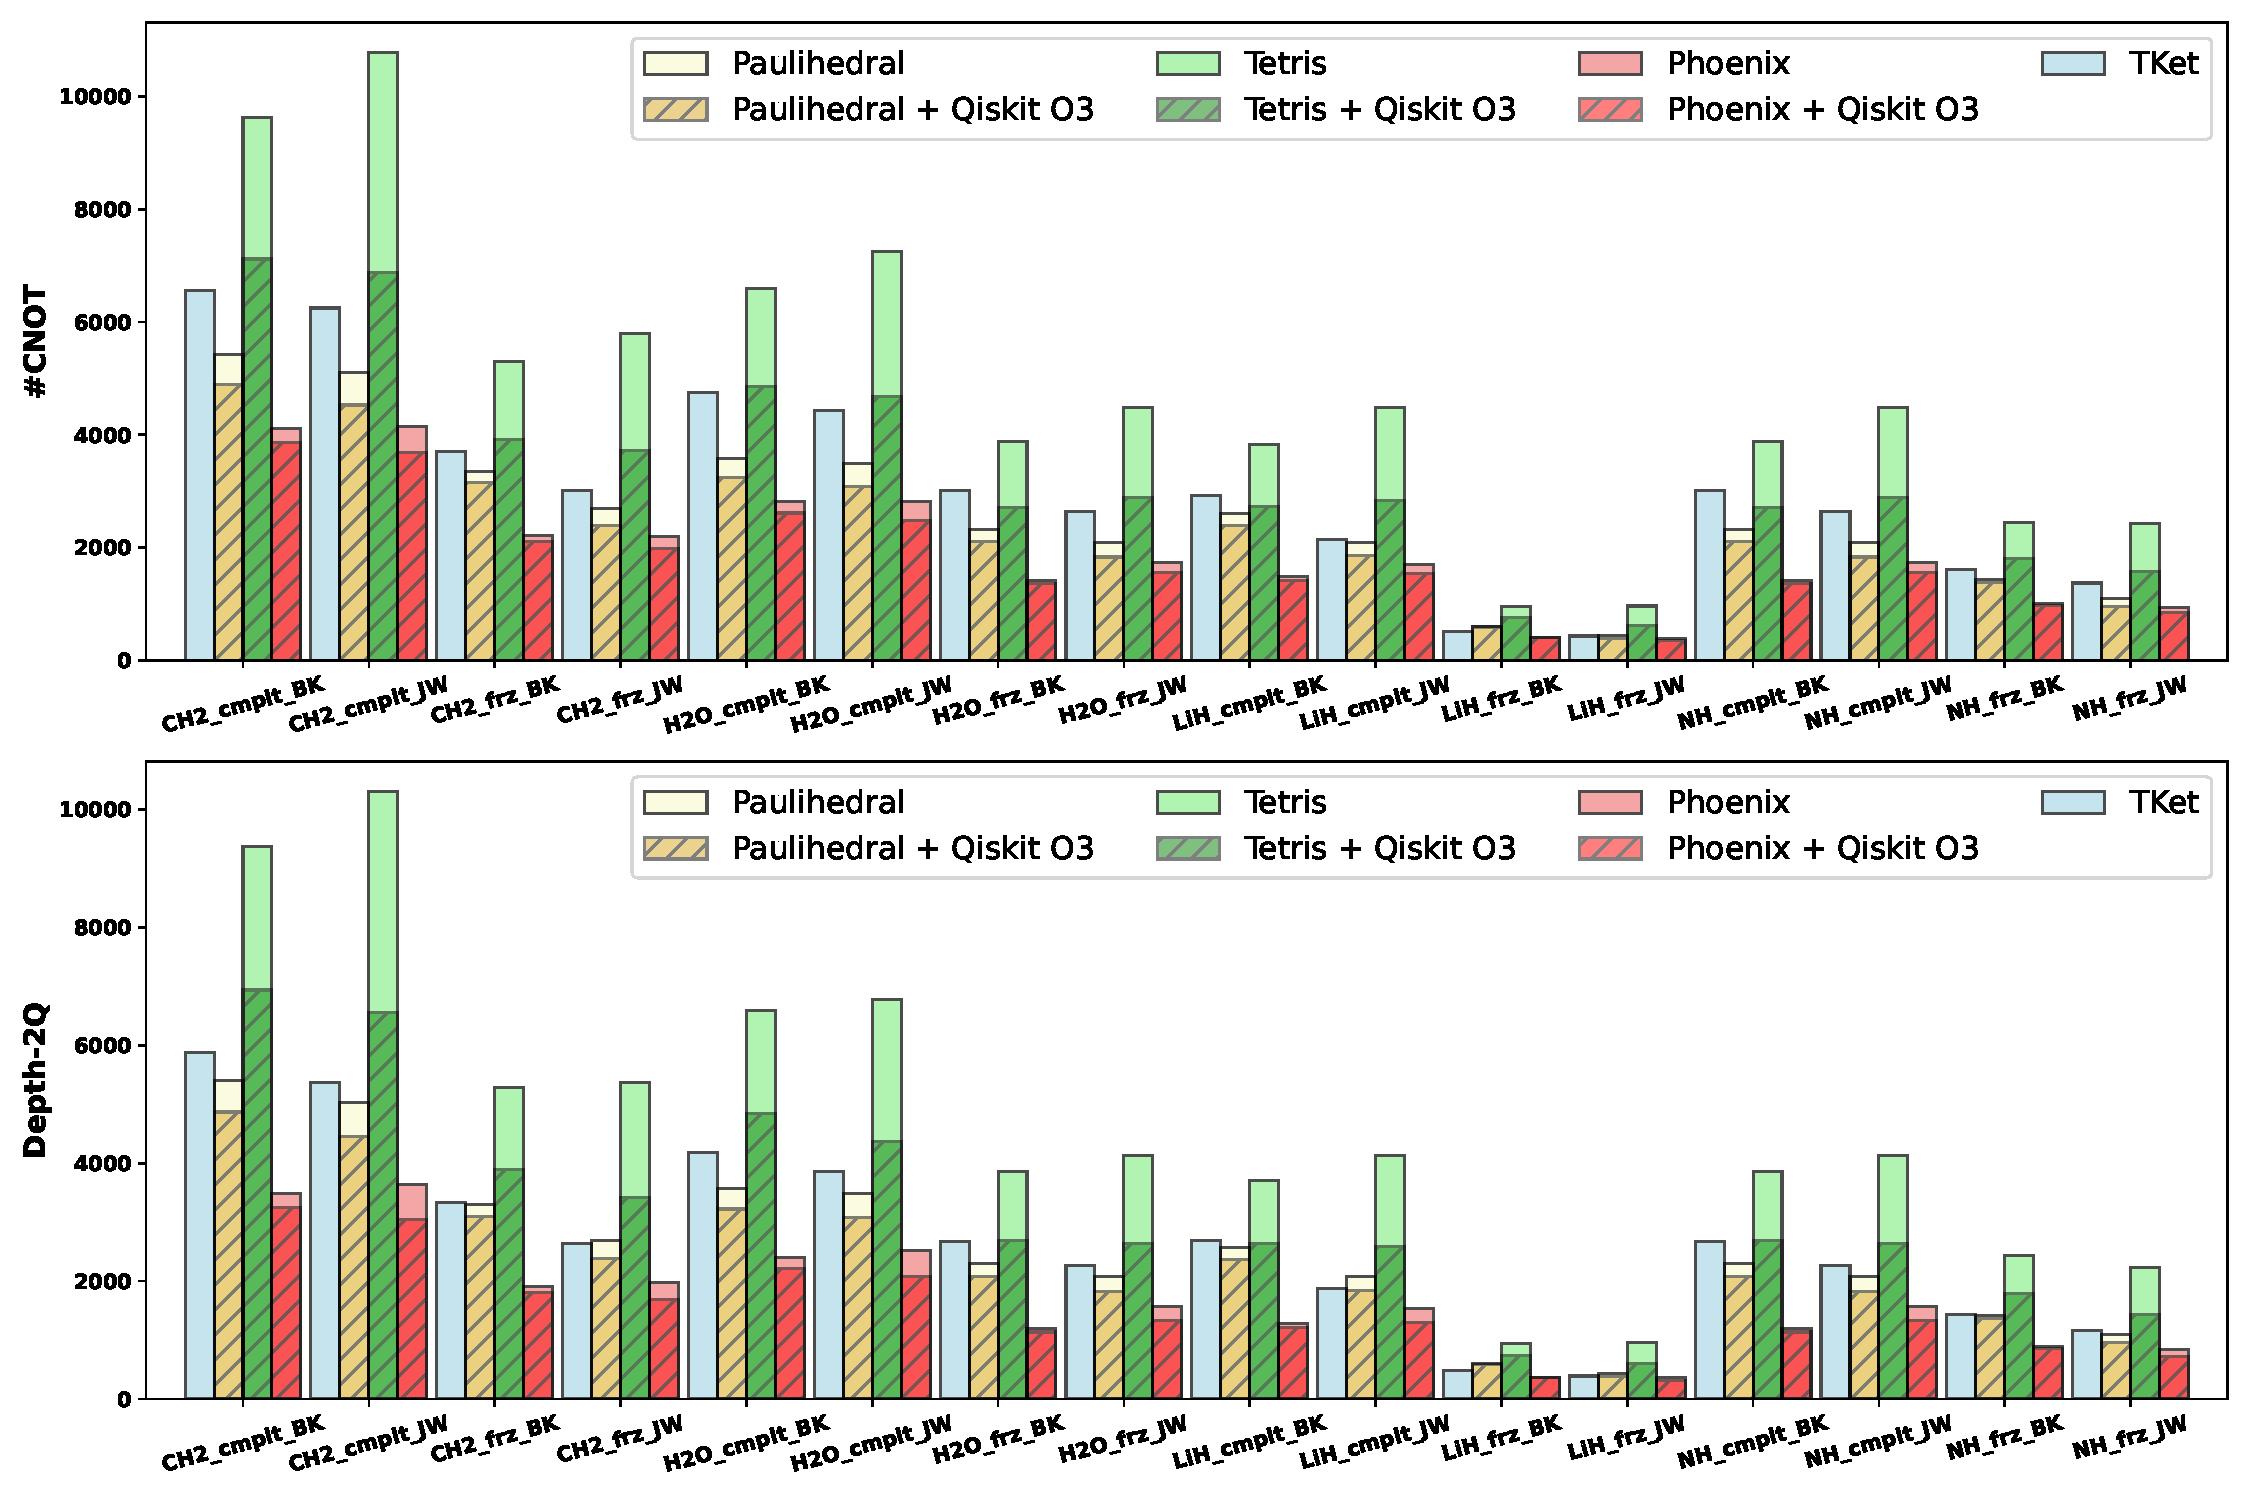
\includegraphics[width=\columnwidth]{figures/all2all.pdf}
        \caption{Logical-level compilation (all-to-all topology).}
        \label{fig:all2all}
    \end{figure}

    \begin{table}[tbp]
        \centering
        \caption{Average (Geometric-mean) optimization rates on UCCSD.}
        \scalebox{0.95}{
            \begin{tabular}{|l|c|c|}
    \hline
    \textbf{Compiler}          & \textbf{\#CNOT opt.}                        & \textbf{Depth-2Q opt.}                     \\ 
    \hline
    \tket                       & 33.07\%                                    & 30.14\%                                   \\ 
    \hline
    \paulihedral                & 28.41\%                                    & 29.07\%                                   \\ 
    \hline
    \multirow{2}{*}{\paulihedral\ + O3}    
                               & 25.72\%                                     & 26.3\%                                    \\ 
                               & (-8.54\% v.s. no O3)                 & (-8.60\% v.s. no O3)               \\ 
    \hline
    \tetris                     & 53.66\%                                    & 53.26\%                                   \\ 
    \hline
    \multirow{2}{*}{\tetris\ + O3}         
                               & 36.73\%                                     & 36.37\%                                   \\ 
                               & (-30.94\% v.s. no O3)                & (-31.08\% v.s. no O3)              \\ 
    \hline
    \phoenix                    & 21.15\%                                    & 19.28\%                                   \\ 
    \hline
    \multirow{2}{*}{\phoenix\ + O3}        
                               & 19.56\%                                     & 17.29\%                                   \\ 
                               & (-6.58\% v.s. no O3)                 & (-8.42\% v.s. no O3)               \\ 
    \hline
\end{tabular}
            
        }
        \label{tab:uccsd-avg}        
    \end{table}

    \Cref{fig:all2all} and \Cref{tab:uccsd-avg} illustrates the main benchmarking results regarding logical program synthesis:
    \begin{enumerate}
        \item \phoenix\ significantly outperforms baselines across all benchmarks, with an average 21.15\% and 17.29\% optimization rate\footnote{For example, the \#$ \CNOT $ optimization rate is defined as $\frac{\#\CNOT_\textrm{after}}{\#\CNOT_\textrm{before}}$.} in \#$ \CNOT $ and Depth-2Q, respectively, relative to original circuits. That is mostly attributed to the group-wise BSF simplification mechanism, as \phoenix\ adopts the same IR grouping method as \paulihedral\ and \tetris.
        \item In task of the logical-level synthesis, \tetris\ performs the worst, falling far behind \tket\ and the earlier \paulihedral, let alone \phoenix. This is because \tetris\ focuses primarily on co-optimization techniques to reduce $\SWAP$ gates during qubit routing.
        \item We also compare \paulihedral/\tetris/\phoenix\ with and without \qiskit\ optimization, to evaluate their proposed high-level optimization capabilities. \qiskit\ O3 improves \paulihedral\ and \tetris\ a lot over our work. Therefore, \phoenix's high-level optimization strategy is more impressive and leaves much less gate cancellation workloads to \qiskit\ O3.
    \end{enumerate}


\subsection{Hardware-aware compilation}

    \begin{figure}[tbp]
        \centering
        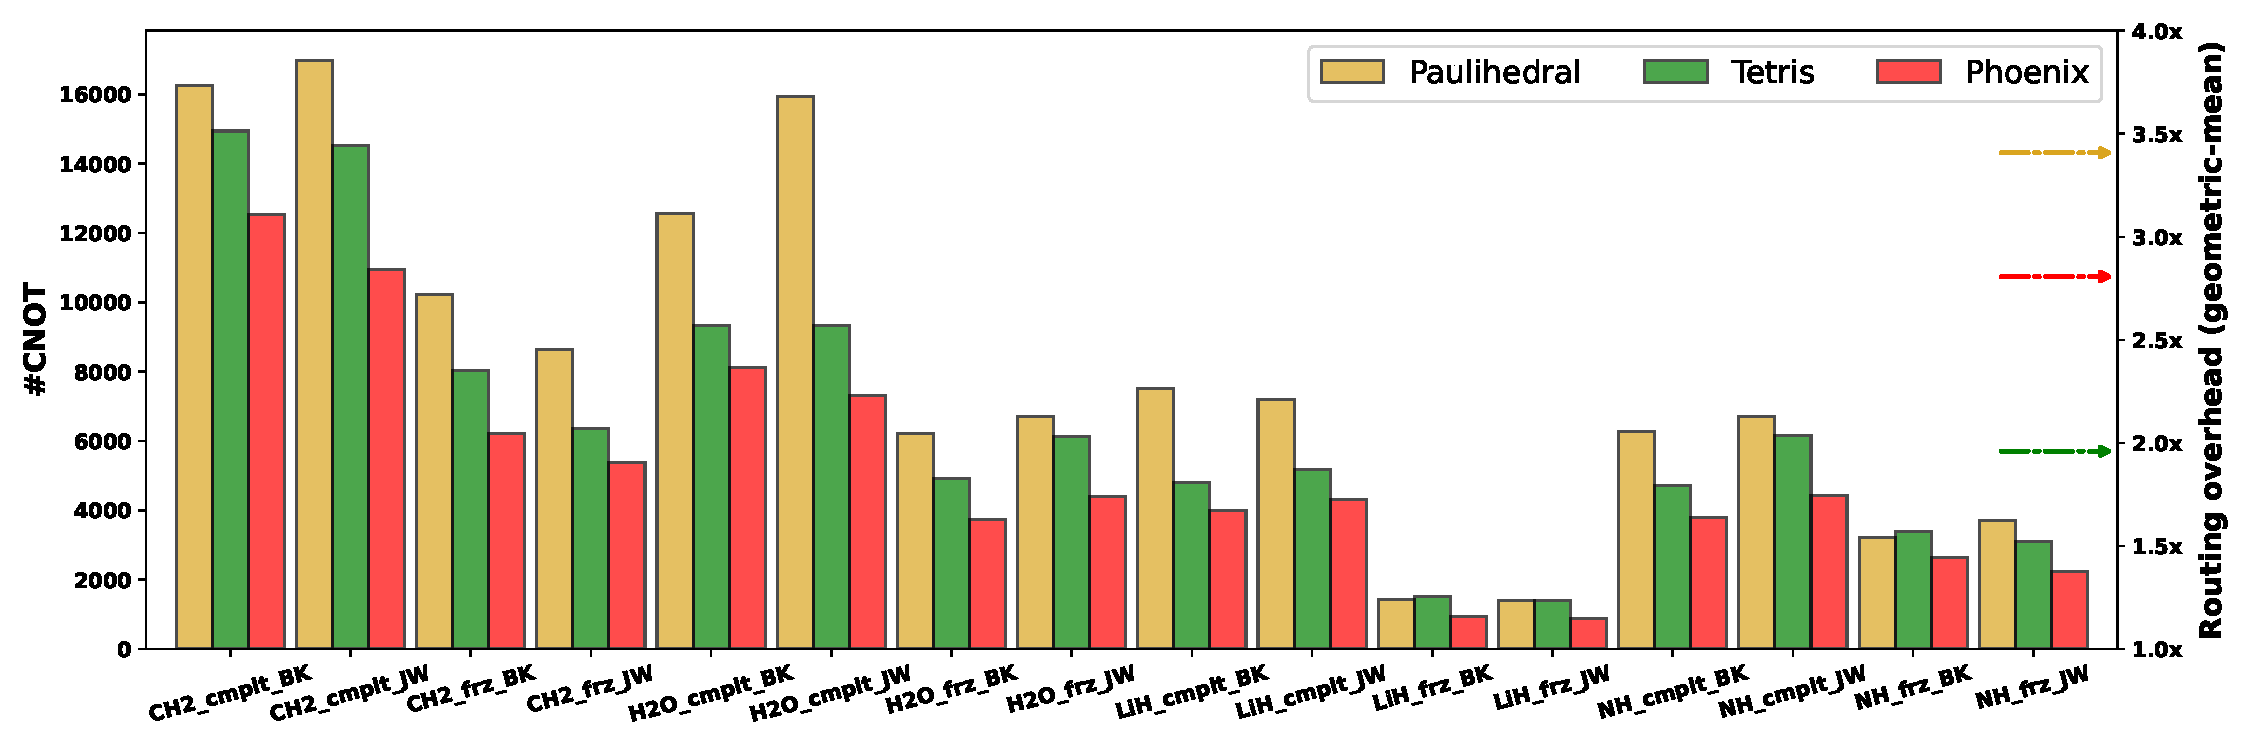
\includegraphics[width=\columnwidth]{figures/num_2q_gates_manhattan.pdf}
        \caption{Hardware-aware compilation on heavy-hex topology. Three dashed lines represent the average multiples of \#$\CNOT$ within circuits after mapping relative to those after logical optimization, for \paulihedral\ (gold), \tetris\ (green), and \phoenix\ (coral), respectively.}
        \label{fig:manhattan}
    \end{figure}


    We choose the heavy-hex topology, specifically a 64-qubit coupling graph corresponding to IBM's Manhattan processor~\cite{mooney2021whole}, as the limited-topology backend to perform hardware-aware compilation. Results are depicted in \Cref{fig:manhattan}. \tket's results are not comparable to \paulihedral/\tetris/\phoenix, so it is not shown in \Cref{fig:manhattan}. Although \phoenix\ focuses primarily on high-level logical program optimization while integrates limited efforts on hardware-aware co-optimization, it still outperforms \paulihedral\ and \tetris\ in terms of \#$ \CNOT $ and Depth-2Q of the ultimate mapped circuits, with an average 35.9\% (22.3\%) and 43.6\% (27.8\%) reduction, respectively, compared to \paulihedral\ (\tetris). 
  
    The consideration of integrating qubit mapping transition overhead into the heuristic IR group ordering functionality in \phoenix\ controls the routing overhead, resulting in 2.8x \#$ \CNOT $ on average. That is better than \paulihedral\ and worse than \tetris, since the latter specially exploits \#$\CNOT$ cancellation opportunities for $ \SWAP $-based routing. 

    
    Consequently, even for hardware mapping on limited-topology devices, \phoenix\ effectively controls qubit routing overhead and ultimately surpasses co-design local optimization strategies.


\subsection{Comparison in diverse ISAs}


    % \begin{figure}[tbp]
    %     \centering
    %     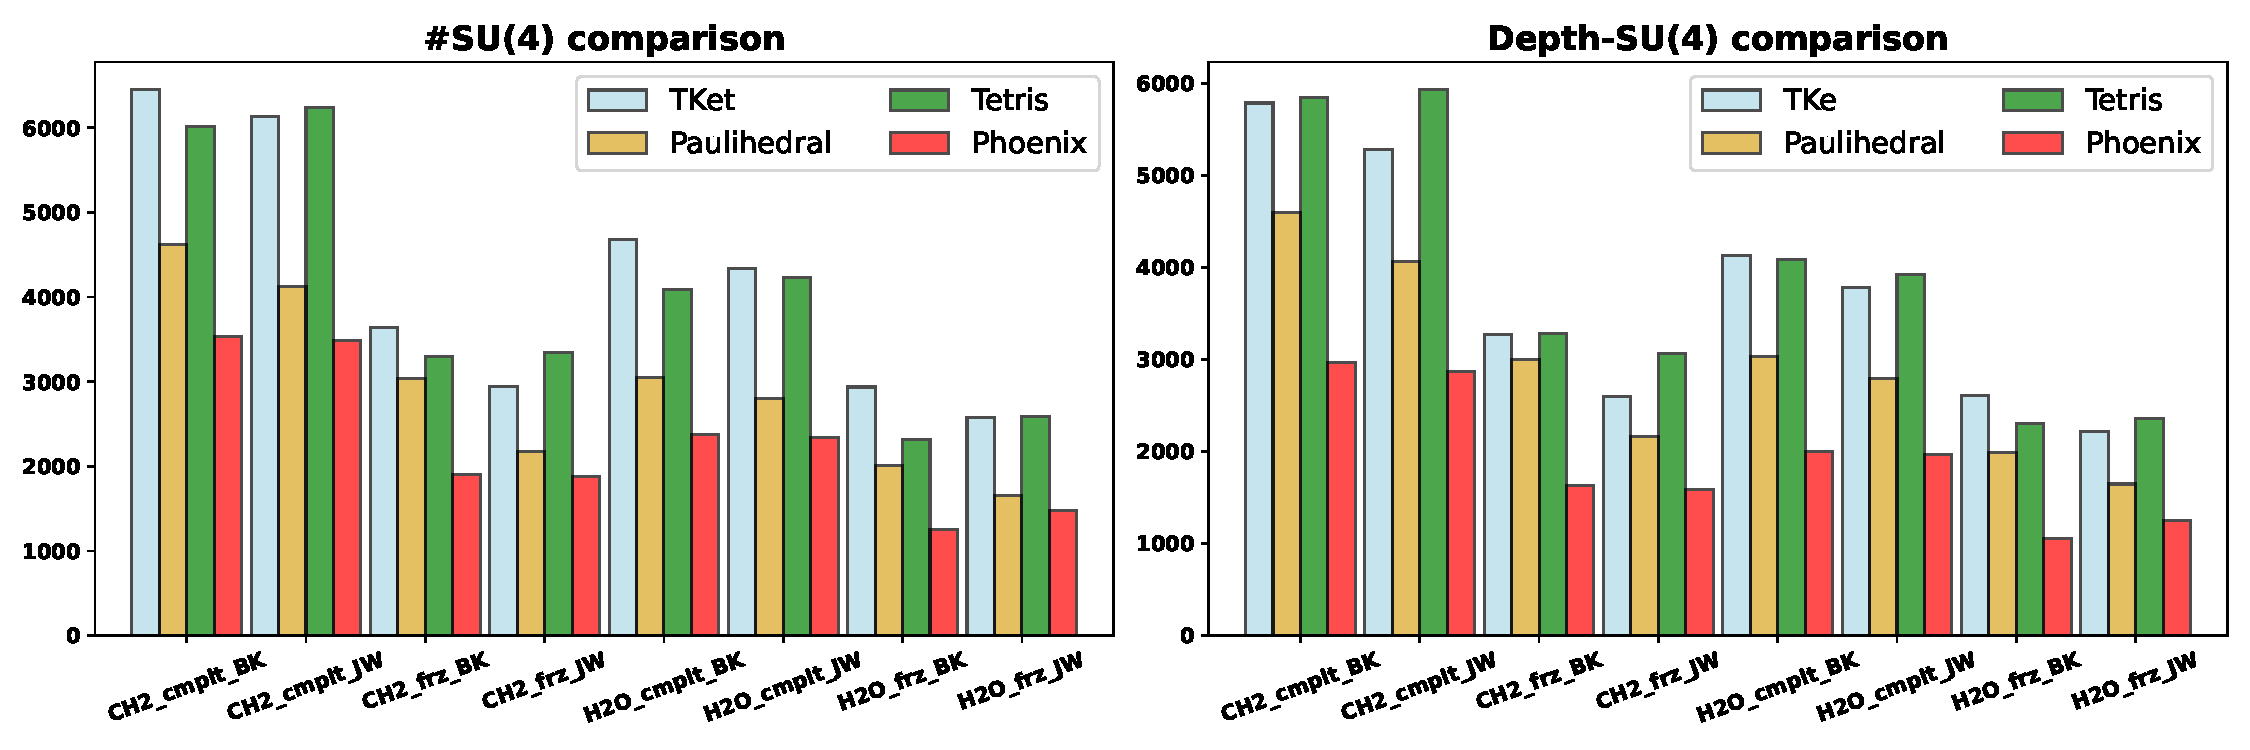
\includegraphics[width=\columnwidth]{figures/su4_comparison.pdf}
    %     \caption{Compilation targeting SU(4) ISA. Part of results are shown for brevity.}
    %     \label{fig:su4-isa}
    % \end{figure}
    \begin{table*}[tbp]
        \centering
        \caption{Comparison for diverse ISAs with all-to-all and limited-topology.}
        \begin{tabular}{|l|c|c|c|c|c|c|c|c|}
    \hline
     & \multicolumn{2}{|c|}{\textbf{CNOT ISA (all-to-all)}} & \multicolumn{2}{|c|}{\textbf{SU(4) ISA (all-to-all)}} & \multicolumn{2}{|c|}{\textbf{CNOT ISA (heavy-hex)}} & \multicolumn{2}{|c|}{\textbf{SU(4) ISA (heavy-hex)}} \\ \hline
    \textbf{\phoenix's opt. rate} & {\#CNOT} & {Depth-2Q} & {\#SU(4)} & {Depth-2Q} & {\#CNOT} & {Depth-2Q} & {\#SU(4)} & {Depth-2Q} \\ \hline
    \phoenix\ v.s. \tket          & 63.93\%       & 63.96\%           & \textbf{56.12\%} & \textbf{54.21\%} & \textbf{40.79\%} & \textbf{48.51\%} & 44.44\%       & 50.65\%           \\ \hline
    \phoenix\ v.s. \paulihedral   & 82.21\%       & 73.29\%           & \textbf{75.69\%} & \textbf{65.18\%} & 62.63\%         & 54.92\%         & \textbf{39.97\%} & \textbf{35.02\%} \\ \hline
    \phoenix\ v.s. \tetris        & 57.58\%       & 53.01\%           & \textbf{56.63\%} & \textbf{50.54\%} & 76.27\%         & 71.47\%         & \textbf{62.44\%} & \textbf{58.66\%} \\ \hline
\end{tabular}
    
        \label{tab:isa}
    \end{table*}

    Quantum instruction set architecture (ISA), or the native gate set in a narrow sense, serves as a contract between software and hardware implementation. The design of quantum ISA plays a crucial role in the performance of NISQ devices, in which the 2Q gate dominates its hardware accuracy and cost as well as the software expressivity. Although the conventional gate set includes 1Q gates and CNOT-based 2Q gates, recently some works propose integrating complex and continuous 2Q gates into the ISA design, such as the $\mathrm{XY}(\theta)$ gate family by Rigetti Computing~\cite{abrams2020implementation}, the fractional gates on IBM's Heron processors\footnote{\footnote{\href{https://www.ibm.com/quantum/blog/fractional-gates}{https://www.ibm.com/quantum/blog/fractional-gates}}}, and the AshN gate scheme~\cite{chen2024one} considering all possible 2Q gates within the $\SUfour$ group as the quantum ISA.    
    
    Therefore, we further compare \phoenix\ with baselines in different quantum ISAs, to showcase that \phoenix's ISA-independent synthesis strategies proves to be a generally powerful optimization engine accommodating diverse ISAs.
    
    Without loss of generality, we consider the most expressive $\SUfour$ ISA with all-to-all and heavy-hex qubit topologies, respectively, in addition to the benchmarking in $ \CNOT $ ISA above. For logical-level compilation, \phoenix\ can directly generate $ \SUfour $-based circuits through its BSF simplification algorithm, while for baselines (\paulihedral\ and \tetris\ are equipped with \qiskit\ O3 by default) an extra \dquote{rebase} (or \dquote{transpile}) procedure is required to convert the $ \CNOT $-based circuits to $ \SUfour $-based ones; for hardware-aware compilation, all compilers require the rebase procedure, following the \qiskit\ O3 hardware-aware compilation pass. Detailed outcomes are summarized in \Cref{tab:isa}, wherein we highlight the geometric-mean relative optimization rates of \phoenix compared to baselines' results.
    % \begin{enumerate}
    %     \item Again, \phoenix\ significantly outperforms baselines when targeting $ \SUfour $ ISA. 
    %     \item The optimization rates relative to baselines are more impressive than those in $ \CNOT $ ISA, despite the baselines incorporating sophisticated optimization techniques specifically designed for the $ \CNOT $ ISA. For instance, the multiple of \phoenix's \#2Q relative to \paulihedral's in $ \CNOT $ ISA is 82.21\% (62.63\%), whereas this value decreases to 75.69\% (39.97\%) in $ \SUfour $ ISA for hardware-agnostic (hardware-aware) compilation. 
    %     \item One exception is the hardware-aware compilation comparison with \tket, as \tket's hardware-aware compilation in $ \CNOT $ ISA generates much larger 2Q gate count and circuit depth than other compilers, and there are many 2Q subcircuit fusing opportunities such that the rebased circuits involves much fewer $ \SUfour $ gates.
    % \end{enumerate}

    Again, \phoenix\ significantly outperforms baselines when targeting $ \SUfour $ ISA. The optimization rates relative to baselines are more impressive than those in $ \CNOT $ ISA, despite the baselines incorporating sophisticated optimization techniques specifically designed for the $ \CNOT $ ISA. For instance, the multiple of \phoenix's \#2Q relative to \paulihedral's in $ \CNOT $ ISA is 82.21\% (62.63\%), whereas this value decreases to 75.69\% (39.97\%) in $ \SUfour $ ISA for hardware-agnostic (hardware-aware) compilation. One exception is the hardware-aware compilation comparison with \tket, as \tket's hardware-aware compilation in $ \CNOT $ ISA generates much larger 2Q gate count and circuit depth than other compilers, and there are many 2Q subcircuit fusing opportunities such that the rebased circuits involves much fewer $ \SUfour $ gates.


% \subsection{Breakdown analysis}

% \textbf{Lookahead effect}


% \textbf{Clifford subcircuit generated by BSF simplification algorithm}


% \textbf{Weight for routing-aware ordering}


\subsection{QAOA benchmarking}

    \begin{figure}[tbp]
        \centering
        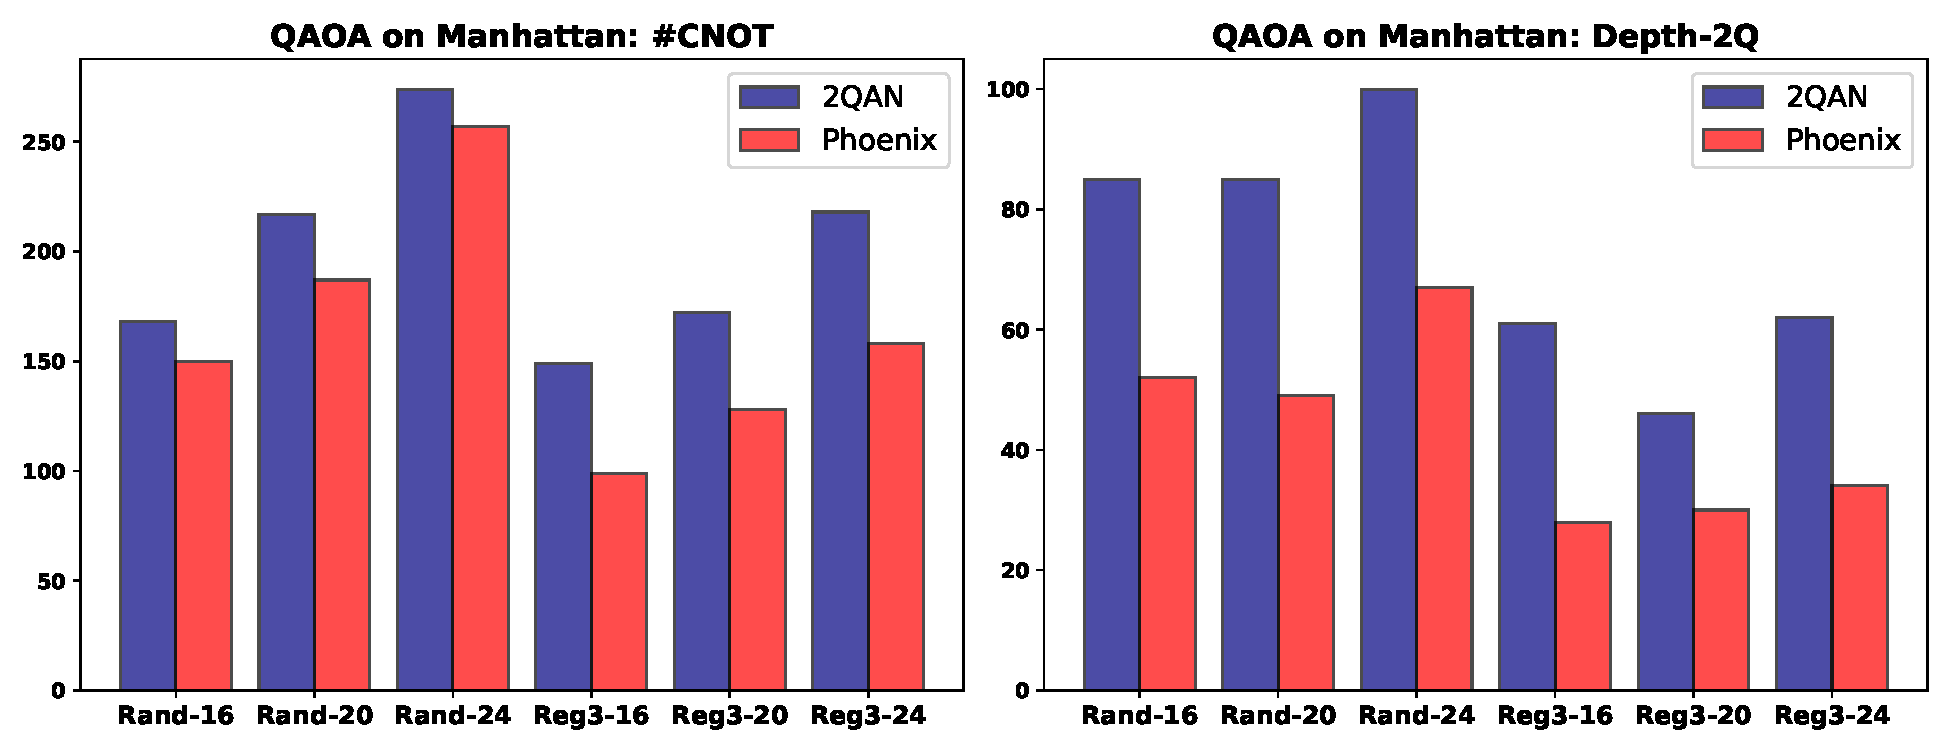
\includegraphics[width=\columnwidth]{figures/qaoa.pdf}
        \caption{QAOA benchmarking}
        \label{fig:qaoa}
    \end{figure}



    \begin{table}[btp]
        \centering
        \caption{QAOA benchmarking versus 2QAN.}
        \setlength{\tabcolsep}{3.8pt}
        \scalebox{0.78}{
            \begin{tabular}{|l|r|r|r|r|r|r|r|r|r|r|}
    \hline
    \multicolumn{2}{|c|}{QAOA} & \multicolumn{2}{c|}{\#CNOT} & \multicolumn{2}{c|}{Depth-2Q} & \multicolumn{2}{c|}{\#SWAP} & \multicolumn{2}{c|}{Routing overhead} \\ 
    \hline
    Bench. &  \#Pauli & 2QAN & Phoenix & 2QAN & Phoenix & 2QAN & Phoenix & 2QAN & Phoenix \\
    \hline
    Rand-16 & 32 & 168 & 150 & 85 & 52 & 37 & 29 & 2.62 & 2.34 \\
    \hline
    Rand-20 &  40 & 217 & 187 & 85 & 49 & 47 & 39 & 2.71 & 2.34 \\
    \hline
    Rand-24 &  48 & 274 & 257 & 100 & 67 & 63 & 56 & 2.85 & 2.68 \\
    \hline
    Reg3-16 &  24 & 149 & 99 & 61 & 28 & 44 & 17 & 3.10 & 2.06 \\
    \hline
    Reg3-20 &  30 & 172 & 128 & 46 & 30 & 46 & 23 & 2.87 & 2.13 \\
    \hline
    Reg3-24 &  36 & 218 & 158 & 62 & 34 & 62 & 30 & 3.03 & 2.19 \\
    \hline
    \multicolumn{2}{|c|}{\emph{Avg. improv.}} & \multicolumn{2}{c|}{-16.7\%} & \multicolumn{2}{c|}{-40.8\%} & \multicolumn{2}{c|}{-29.41\%} & \multicolumn{2}{c|}{-16.59\%} \\
    \hline
\end{tabular}
    
        }
        \label{tab:qaoa}
    \end{table}

    For QAOA benchmarking, we focus on the the performance in hardware-aware compilation, since the 2Q gate count cannot be reduced and minimizing circuit depth is trivial in logical-level compilation, as both \twoqan\ and \phoenix\ can generate depth-optimal QAOA circuits at the logical level at the in our field test. \Cref{fig:qaoa} and \Cref{tab:qaoa} illustrate compilation results on heavy-hex topology, across six representative QAOA programs corresponding to both random graphs (each node with degree 4) and regular (each node with degree 3) graphs, with qubit sizes of 16, 20, and 24. \phoenix\ outperforms \twoqan\ across all benchmarks in all metrics (e.g., \#$ \CNOT $, \#$ \SWAP $), especially in Depth-2Q, with an average 40.8\% reduction compared to \twoqan. These results further demonstrate the effectiveness of the routing-aware IR group ordering method in \phoenix.

\subsection{Algorithmic error analysis}


    \begin{figure}[tbp]
        \centering
        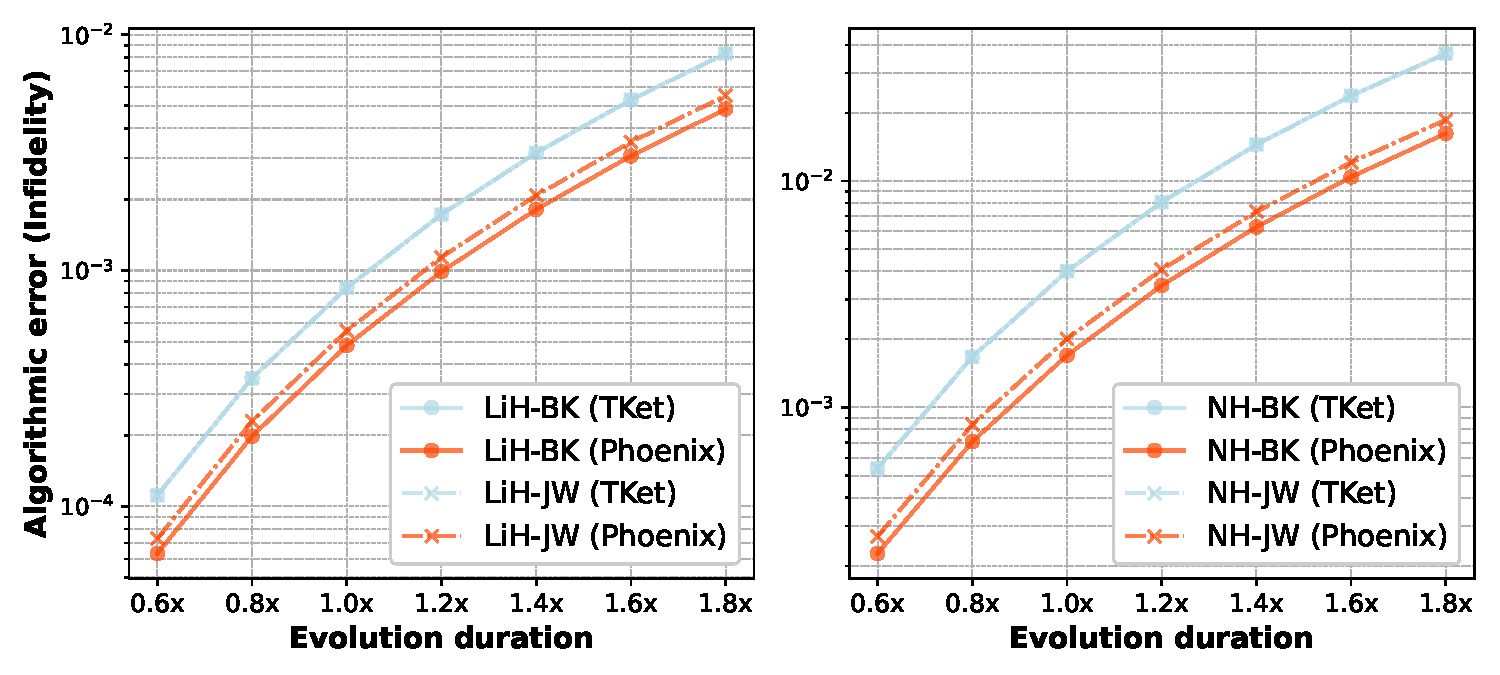
\includegraphics[width=\columnwidth]{figures/algo_err.pdf}
        \caption{Algorithmic error comparison of \LiH\ and \NH\ simulation.  }
        \label{fig:algo-err}
    \end{figure}

    We further highlight the advantage of \phoenix\ in reducing algorithmic errors for VQA programs, which limits the best accuracy of practical VQA's outcomes when executing on noisy hardware. From UCCSD benchmarks, we select those with qubit sizes no more than 10 for evaluation, given the matrix computation capabilities of standard PCs. We rescale the coefficients of Pauli strings to control their algorithmic errors within the range of 0.00005 to 0.01, which corresponds to different-scale evolution durations of molecular simulation, as suggested in \Cref{fig:algo-err}. In contrast to \tket, \phoenix\ typically leads to lower algorithmic errors for both JW and BK encoding schemes. Although this improvement is program-specific, it is more significant for Pauli string patterns of BK than those of JW, with 57\% (42.7\%) and 49.5\% (34.1\%) for \NH\ (\LiH) simulation, respectively. The algorithmic errors resulting from \paulihedral\ and \tetris\ are comparable to \phoenix\ and are not shown in \Cref{fig:algo-err}, as they adopt the same Pauli string blocking approach. As a result, the impressive algorithmic error reduction effect of \phoenix\ further pushes toward the quantum advantage on computational chemistry problems.


\subsection{Fidelity analysis}


\ZY{TODO or to delete}




%%%%%%%%%%%%%%%%%%%%%%%%%%%%%%%%%%%%%%%%%%%%%%%%%%%%%%%%%
% Conclustion and Outlook
%%%%%%%%%%%%%%%%%%%%%%%%%%%%%%%%%%%%%%%%%%%%%%%%%%%%%%%%%

\section{Conclusion and Outlook}

    \ZY{Summary of our work}






%%%%%%%%%%%%%%%%%%%%%%%%%%%%%%%%%%%%%%%%%%%%%%%%%%%%%%%%%
% Acknowledgement
%%%%%%%%%%%%%%%%%%%%%%%%%%%%%%%%%%%%%%%%%%%%%%%%%%%%%%%%%
% \section*{Acknowledgement}
% ...

%%%%%%%%%%%%%%%%%%%%%%%%%%%%%%%%%%%%%%%%%%%%%%%%%%%%%%%%%
% Reference
%%%%%%%%%%%%%%%%%%%%%%%%%%%%%%%%%%%%%%%%%%%%%%%%%%%%%%%%%
\newpage
\bibliographystyle{IEEEtran}
\bibliography{reference}


%%%%%%%%%%%%%%%%%%%%%%%%%%%%%%%%%%%%%%%%%%%%%%%%%%%%%%%%%
% Appendix
%%%%%%%%%%%%%%%%%%%%%%%%%%%%%%%%%%%%%%%%%%%%%%%%%%%%%%%%%


% \appendix{...}




\end{document}
